% !TeX spellcheck = en_US
\chapter{The IceAct Model in \geant}

\section{\geant}
\geant is a multi-purpose simulation framework for the passage of particles trough matter, written in \textit{C++} and developed by the \geant Collaboration at CERN. It includes physics models, geometry, tracking, hits, and digitization and thus allows a detailed simulation and response analysis for particle detectors in many application fields like particle and accelerator physics, space engineering or medical science. In the framework's source some basic and advanced use cases are implemented and provided as examples. The toolkit is built up of multiple categories (or modules) using each other (cf. figure \ref{geant4:categories}). \cite{geant4}

\begin{wrapfigure}{r}{0.5\textwidth}
	\centering
	
\includegraphics[width=0.5\textwidth]{Geant4Logo.png}
	\caption[\geant Logo]{\textbf{\geant logo.} \cite{geant4:logo}}	
\end{wrapfigure}

\begin{figure}[h]
	\centering
	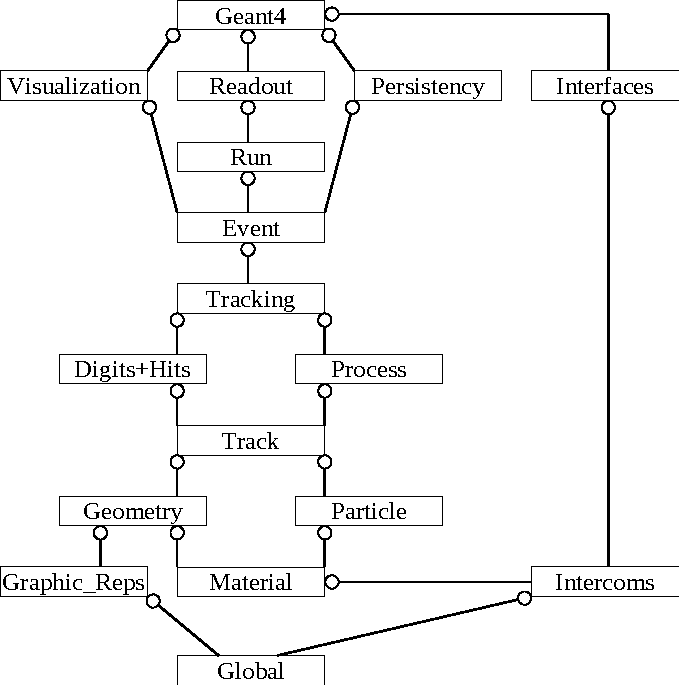
\includegraphics[width=0.6\textwidth]{Geant4ConceptDiagram.pdf}
	\caption[\geant category diagram]{\textbf{Diagram of relationships between \geant categories. \cite{geant4}} The circles represent a \enquote{using} relation. The category with the circle next to the box uses the linked one.}	
	\label{geant4:categories}
\end{figure}

Especially for the use case of IceAct \geant is capable of simulating Cherenkov (optical) photons, material properties like transmission, reflection, and refraction, as well as detection efficiency properties of the SiPMs.

Since this thesis is about an approach of an all-encompassing telescope simulation, \geant provides all major possibilities to get a distinct analysis of the entire optical system of IceAct.

\subsection{FAMOUS telescope simulation}
The fluorescence telescope FAMOUS\footnote{\textbf{F}irst \textbf{A}uger \textbf{M}ulti-pixel
photon counter camera for the \textbf{O}bservation of \textbf{U}ltra-high-energy air \textbf{S}howers} for the Pierre Auger Observatory in Argentina is developed at RWTH Aachen to measure fluorescence light originating from ultra-high-energy cosmic rays (UHECR) by using Silicon Photomultipliers (SiPMs). Withing the development, a detailed \geant simulation has been elaborated. \cite{famous:sim_github,famous:sim_github} The telescope design of FAMOUS is very similar since the detection technique and the optics system is basically the same. Therefore, the IceAct telescope simulation is heavily based on this FAMOUS \geant framework. A detailed discourse and a summary of previous analyses can be found in \cite{famous:niggemann}.

\section{Materials}

For an optical device, the material that the light should pass has to be chosen deliberately. Especially the transmission properties, processability, and for IceAct in particular the resistance against harsh weather conditions are of interest.

The glass plate on top of IceAct is made of SCHOTT BOROFLOAT\textsuperscript{\textregistered} 33 borosilicate glass with a thickness of \SI{2+-0.2}{\milli\meter} and a diameter of \SI{650.3+-1}{\milli\meter}. \cite{iceact:borosilicate:datasheet}

\todo{Borosilicate refractive index with spline}

\todo{PMMA refractive index with sellmeier}




\cite{iceact:sellmeier}

\begin{figure}[h]
	\centering
	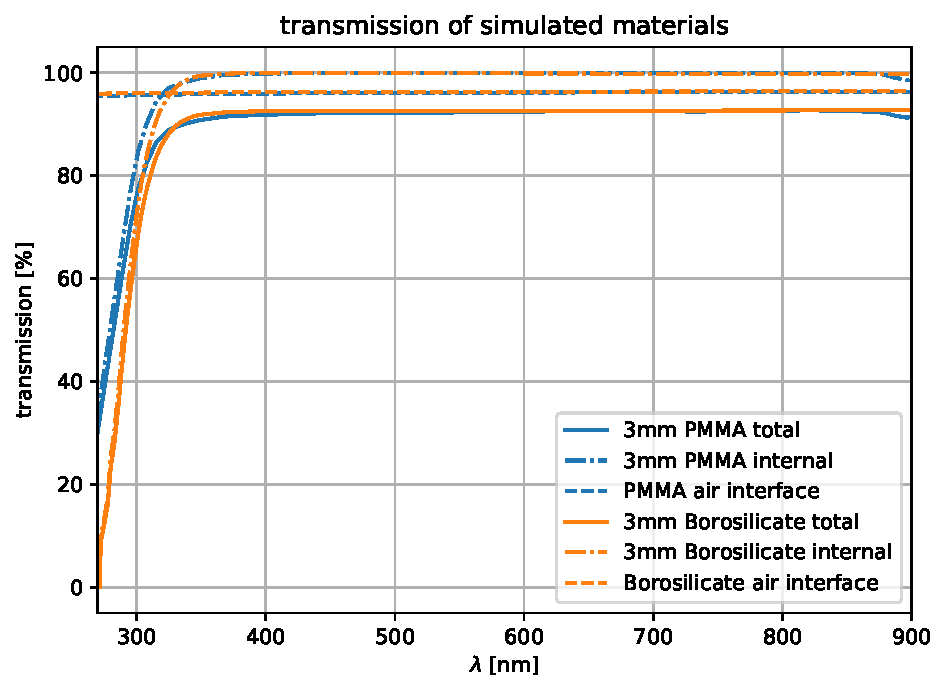
\includegraphics[width=0.8\textwidth]{material/transmission.pdf}
	\caption[Transmission of used materials]{\textbf{Transmission functions of materials used in the simulation.} The total transmission function is the product of internal and two interface transmissions which is evaluated for a perpendicularly incident particle in this plot. Thus, the solid lines represent a complete (perpendicular) transition through a \SI{3}{\milli\meter} thick layer of the respective material.}
	\label{iceact:model:material:transmission}	
\end{figure}

\begin{figure}[h]
	\centering
	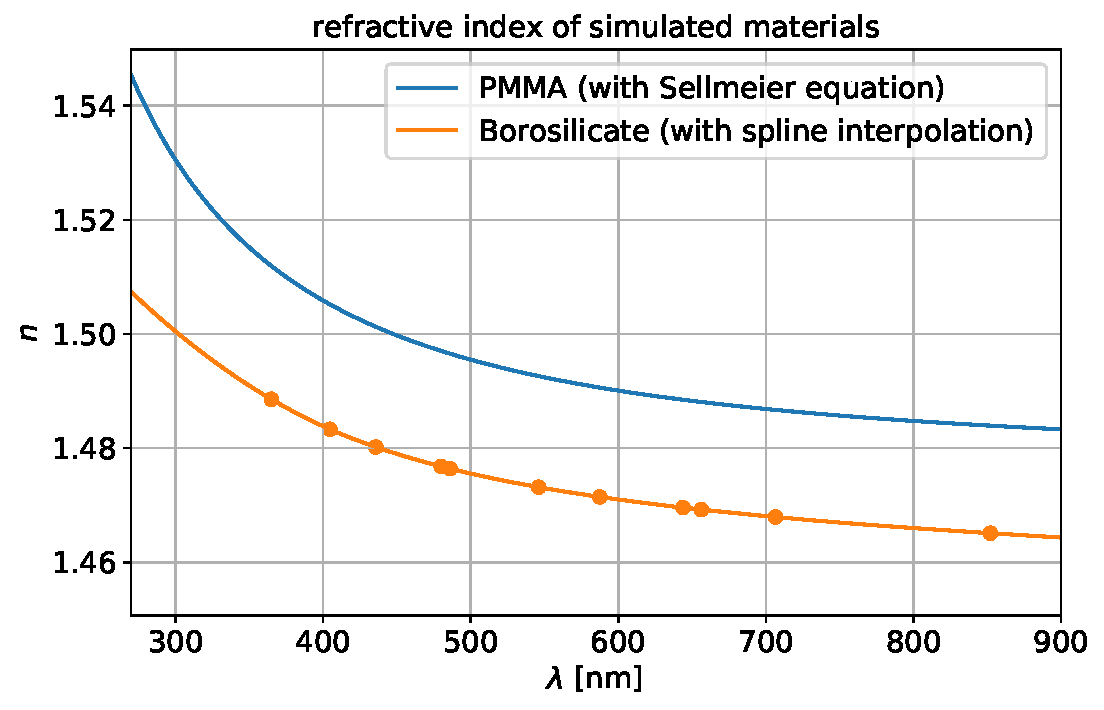
\includegraphics[width=0.8\textwidth]{material/refractive_index.pdf}
	\caption[Refractive index of used materials]{\textbf{Refractive index of materials used in the simulation.} The dispersion is calculated by evaluating the Sellmeier equation introduced in this section.}
	\label{iceact:model:material:refractive_index}	
\end{figure}

The tube, back plane and other coating surfaces are simulated as \enquote{dummy} material with no reflection or transmission parameters. A particle hits those surfaces is absorbed and not considered any further.

\section{Optics}

In the following section the four optical components of the IceAct \geant model are discussed. To have a first glimpse of the model, see figure \ref{iceact:model:cut}.
\begin{figure}[h]
	\centering
	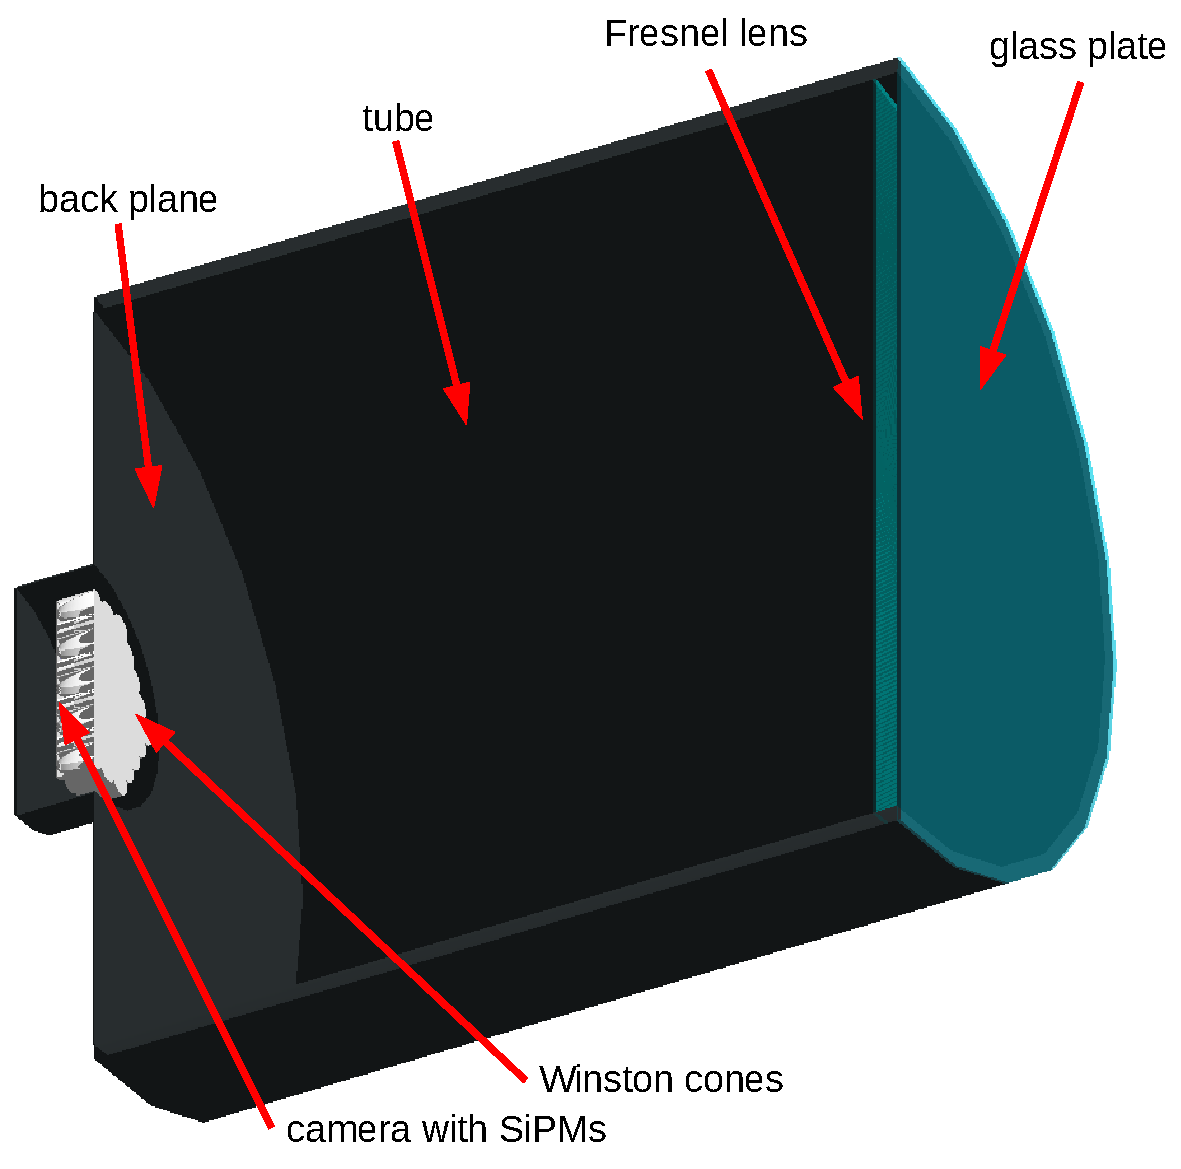
\includegraphics[width=0.6\textwidth]{IceActGeant4Model.pdf}
	\caption[IceAct \geant model]{\textbf{The IceAct \geant model.} Cross-sectional sketch of the IceAct optics in \geant with all simulated components. They are described in detail in \cref{iceact:model:fresnellens,iceact:model:camera,iceact:model:glassplate}.}
	\label{iceact:model:cut}	
\end{figure}

\subsection{Glass Plate}\label{iceact:model:glassplate}

\todo{glass plate}

\subsection{Fresnel Lens}\label{iceact:model:fresnellens}

\begin{figure}[h]
	\centering
	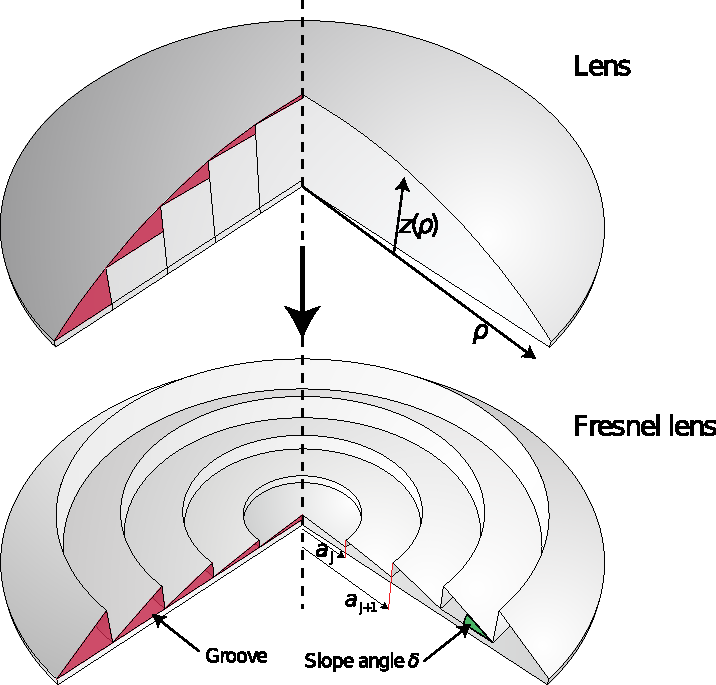
\includegraphics[width=0.5\textwidth]{FresnelVsNormalLens.pdf}
	\caption[Comparison conventional vs. Fresnel lens]{\textbf{Comparison between a conventional \enquote{thick} lens and a Fresnel lens. \cite{famous:eichler}} For the functionality of a lens the radius-dependent sagitta function $z(\rho)$ is crucial. To get rid of the bulky material of a conventional lens, the Fresnel lens is divided into annular \enquote{prisms} called \enquote{grooves}. The slope angle $\delta$ of each groove is a local approximation of the sagitta function to ensure the imaging capability.}
	\label{iceact:model:fresnelvsthick}	
\end{figure}

\begin{figure}[h]
	\centering
	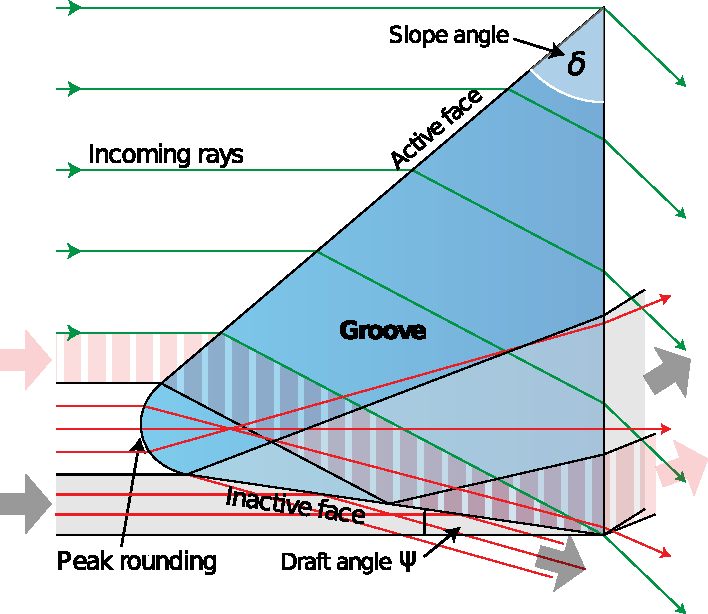
\includegraphics[width=0.5\textwidth]{FresnelGroove.pdf}
	\caption[Fresnel groove]{\textbf{Cross-sectional sketch of a Fresnel groove. \cite{famous:eichler}}}
	\label{iceact:model:fresnelgroove}	
\end{figure}

\todo{write}
\cite{famous:eichler}

\subsection{Camera}\label{iceact:model:camera}

\todo{write}

\subsubsection{Winston Cones}

\todo{write}

\subsubsection{Silicon Photomultiplier}

\todo{write}

